\chapter{Dispostivo Walk400h}
\label{chap:Dispostivo_Walk400h}
    \section{Caratteristiche}
    \begin{figure}[htbp]
    \centering
    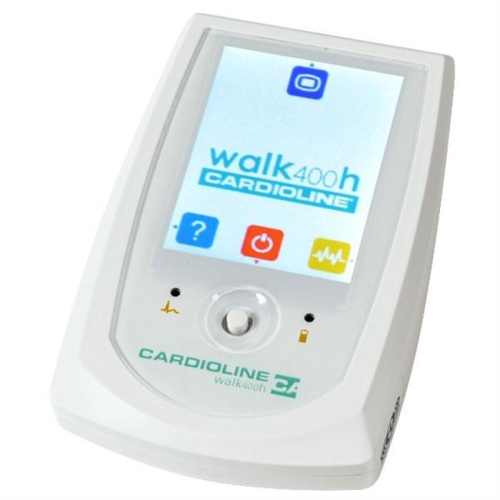
\includegraphics[width=0.4\textwidth]{tesi/img/walk400h.jpg}
    \caption{Dispositivo Walk400h.}
    \label{fig:walk400h_fig}
    \end{figure}
    Il Walk400h è un dispositivo Holter prodotto da Cardioline S.p.a, azienda con sede a Trento, destinato alla registrazione ambulatoriale prolungata del segnale ECG, con una durata di registrazione fino a 7 giorni. Ai fini di questo lavoro non sono di interesse gli aspetti legati all'acquisizione clinica del segnale, quanto piuttosto l'architettura del sistema embedded che gestisce il dispositivo.

    Dal punto di vista architetturale, il Walk400h è basato su un microcontrollore della famiglia \textbf{ARM Cortex-M4} (in particolare \texttt{STM32L471VGT6}), con un firmware eseguito in modalitá \textbf{THUMB}. Il dispositivo integra una memoria Flash di 1 MB utilizzata per il firmware. Per quanto riguarda la memorizzazione dei dati del paziente e aggiornamenti del firmware viene invece usata una \textbf{scheda SD}.

    Il Walk400h espone diversi canali di interazione con l'esterno che costituiscono, da un punto di vista della sicurezza, altrettante superfici di attacco potenziali: l'interfaccia \textbf{USB} per il trasferimento dei dati registrati verso il software di analisi, un'interfaccia \textbf{seriale UART} utilizzata per il logging interno e il meccanismo di aggiornamento basato su \textbf{scheda SD}, quest'ultimo di particolare interesse in quanto rappresenta il principale punto di ingresso di input non fidati nel sistema.

    \section{Reverse Engineering del firmware}
    \label{subsec:firmware_re}
    Il lavoro di reverse engineering del bootloader del Walk400h è stato condotto da Alberici \cite{alberici26}, il quale ha ricostruito la struttura del firmware del dispositivo e ne ha identificato la procedura di aggiornamento. In particolare, tale analisi ha evidenziato come questa procedura non implementi controlli adeguati sull'origine e sull'integrità del nuovo firmware caricato sul dispositivo, aprendo così a un potenziale vettore di attacco per l'esecuzione di codice non autorizzato. Il passo preliminare necessario a questo scopo è stata la ricostruzione dettagliata della struttura del bootloader del Walk400h, volta in particolare a individuare, all'interno del flusso di esecuzione, tutte le componenti del firmware legate al meccanismo di aggiornamento — così da delimitare con precisione le porzioni di codice da sottoporre successivamente a symbolic execution.

    A partire da questo risultato, il presente lavoro si pone l'obiettivo di verificare concretamente lo sfruttabilità di tale mancanza di controlli, tramite l'applicazione di tecniche di symbolic execution alle porzioni di codice coinvolte nel processo di aggiornamento.
        \subsection{Estrazione e caratteristiche del binario}
        Il firmware è stato fornito come immagine binaria raw, priva di metadati (formato eseguibile, simboli di debug, ...). 
        L'analisi statica è stata condotta con \textbf{Ghidra} che ha permesso di determinare le caratteristiche architetturali necessarie per una decompilazione corretta:
        \begin{itemize}[noitemsep]
            \item \textbf{Architettura}: ARM Cortex-M4
            \item \textbf{Set di istruzioni}: Thumb, little-endian
            \item \textbf{Base di caricamento (VMA)}: \texttt{0x08000000}, 
            coerente con il layout tipico della memoria Flash su 
            microcontrollori di questa famiglia
            \item \textbf{Entry point del bootloader}: \texttt{0x08001e34}
        \end{itemize}

        Questi parametri sono stati successivamente riutilizzati come parametri per la fase di decompilazione tramite RetDec, necessaria per produrre una rappresentazione LLVM IR del bootloader analizzabile da KLEE.

    \section{Funzioni critiche identificate}
    \label{subsec:funzioni_critiche}
        A partire dall'entry point, l'analisi del flusso di controllo ha permesso di ricostruire la logica principale del bootloader e di isolare un sottoinsieme di funzioni ritenute critiche per la sicurezza del dispositivo, in quanto ritenute responsabili della gestione dell'aggiornamento firmware e dell'accesso alla SD Card.

        \begin{figure}[H]
        \centering
        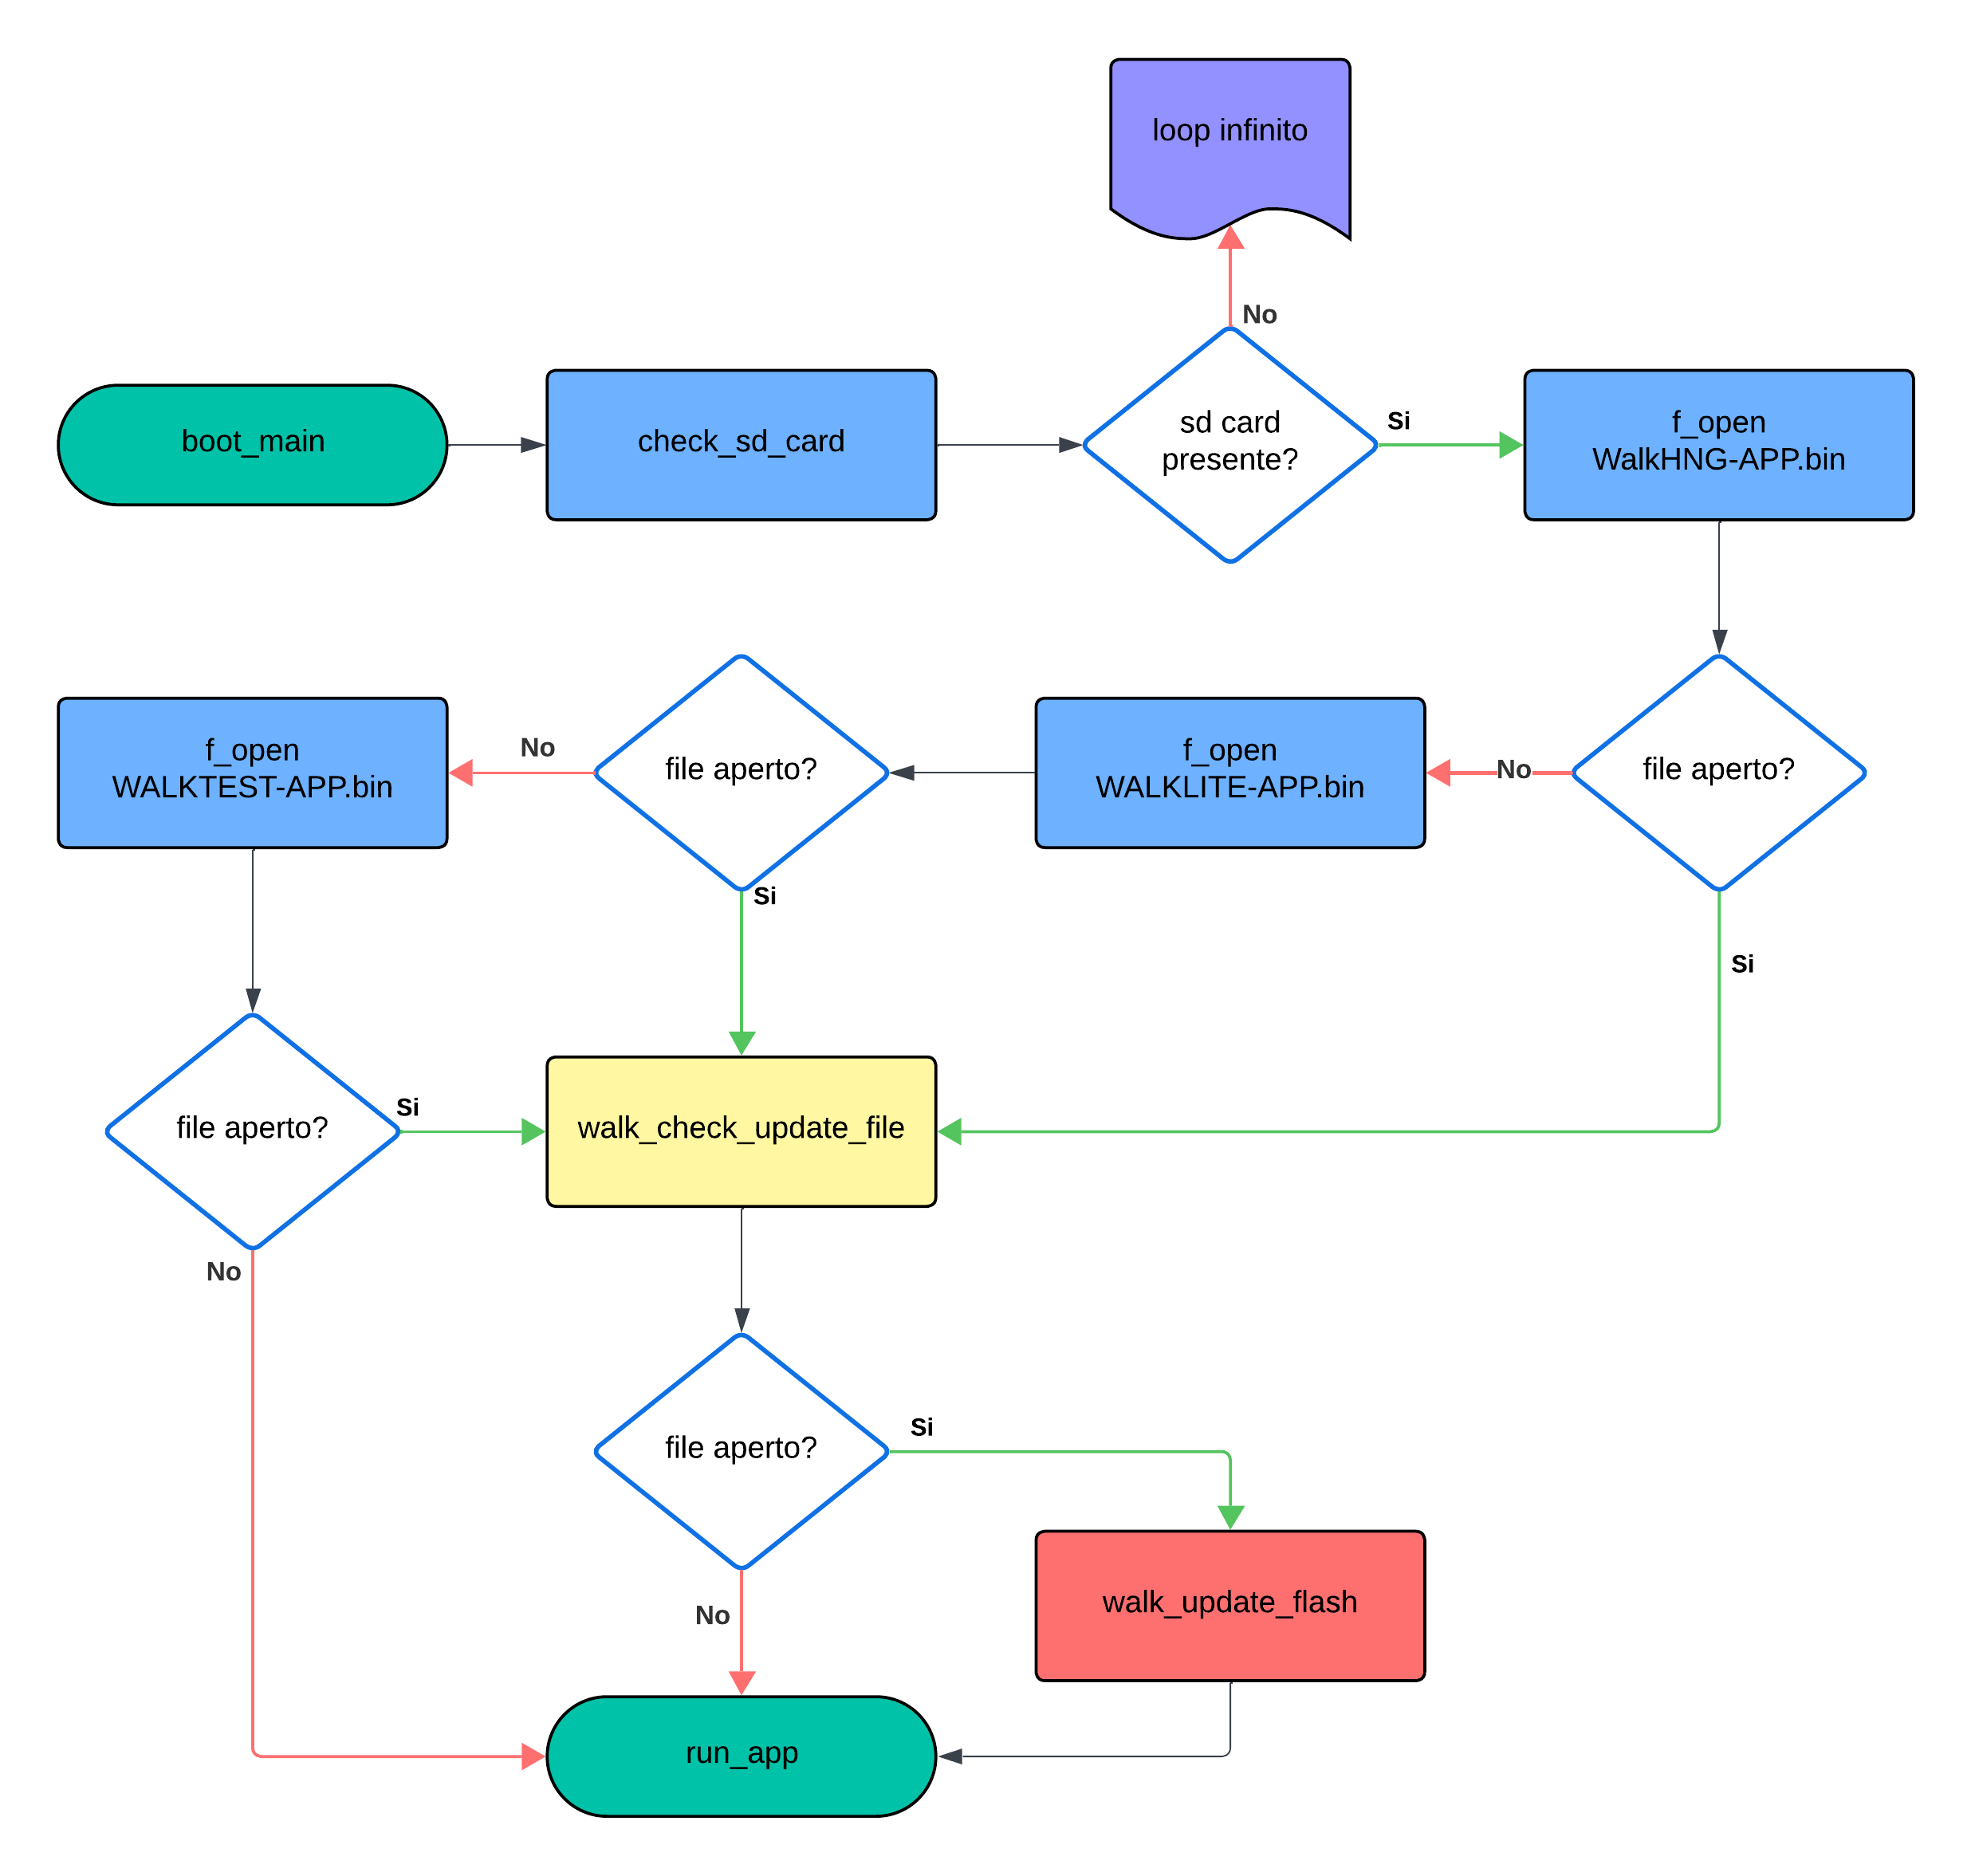
\includegraphics[width=0.8\textwidth]{img/bootloader-flowchart.png}
        \caption{Flowchart semplificato delle funzioni chiave del bootloader del Walk400h.}
        \label{fig:bootloader-flowchart}
        \end{figure}

        \begin{description}
            \item[\texttt{boot\_main}] punto d'ingresso della logica di avvio, 
            responsabile dell'orchestrazione del processo di verifica e 
            aggiornamento del firmware. \\
            \textbf{Criticità}: componente centrale che decide se procedere 
            con l'aggiornamento sulla base dell'esito di alcune verifiche; 
            un errore di logica in questo punto può compromettere 
            l'intero processo di boot.

            \item[\texttt{walk\_check\_update\_file}]
                verifica della validità del file di aggiornamento 
                (\texttt{WALKLITE-APP.bin}) prima che il relativo contenuto venga 
                scritto in memoria Flash. \\
            \textbf{Criticità}: costituisce l'unico punto di controllo tra un 
                file proveniente da un dispositivo di storage removibile e la 
                scrittura in memoria persistente; una validazione insufficiente a 
                questo livello permetterebbe la scrittura di un firmware non 
                verificato.

            \item[\texttt{walk\_update\_flash}]
                scrittura effettiva del nuovo firmware in memoria 
                Flash. \\
                \textbf{Criticità}: operazione privilegiata e irreversibile; un 
                suo utilizzo scorretto (ad esempio raggiungibile bypassando i 
                controlli di \texttt{walk\_check\_update\_file}) comporterebbe la 
                persistenza di codice malevolo sul dispositivo.

        Di particolare interesse è la funzione \texttt{walk\_check\_update\_file}, che costituisce l'unico punto di controllo del file di aggiornamento prima che questo venga considerato valido. Come mostrato in Figura~\ref{fig:walk-check-update-flowchart}, la funzione verifica dapprima l'esistenza del file e che lo spazio disponibile in Flash sia sufficiente per la sua dimensione dichiarata (\texttt{filinfo.size}); in caso contrario, restituisce \texttt{FR\_INT\_ERR}. Superati questi controlli, legge i primi \texttt{0x20} (32) byte del file in un buffer (\texttt{magic}) e ne verifica il contenuto tramite \texttt{mod\_strcmp} e il confronto di quattro byte in coda al buffer (offset \texttt{0x1c}--\texttt{0x1f}): solo se entrambe le condizioni sono soddisfatte il file viene considerato valido (\texttt{FR\_OK}).

        
        
        \begin{figure}[H]
        \centering
        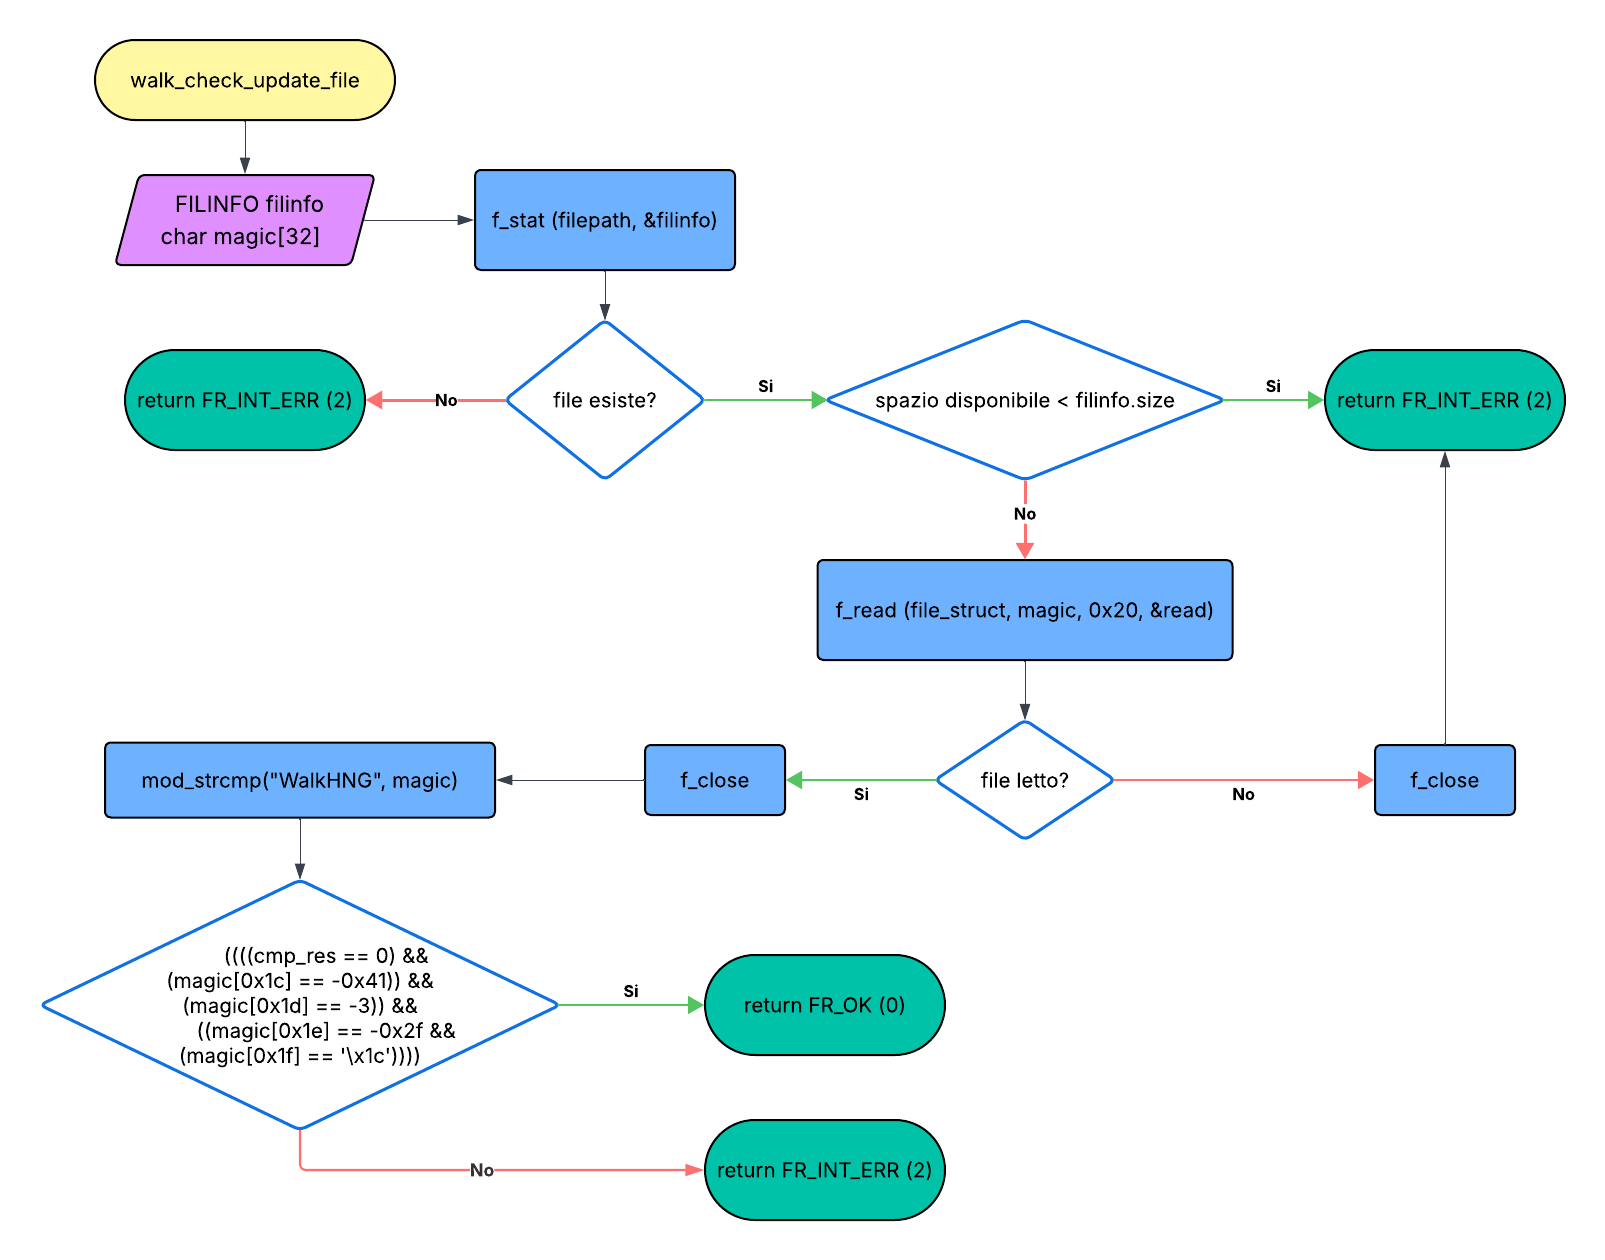
\includegraphics[width=0.8\textwidth]{tesi/img/walk_check_update_file_flowchart.png}
        \caption{Flowchart semplificato della funzione walk\_check\_update\_file.}
        \label{fig:walk_check_update_file_flowchart}
        \end{figure}
        \end{description}
    
    \section{Meccanismi di monitoraggio implementati}
    \label{subsec:meccanismi_di_monitoraggio}
        Nell'ottica di validare i risultati dell'analisi statica condotta in questa sezione e descritta nel lavoro di Alberici~\cite{alberici26}, e per supportare la successiva esplorazione simbolica del medesimo percorso con gli strumenti di analisi utilizzati, sono stati implementati due meccanismi di osservabilità del comportamento del firmware: il primo consente di monitorare i messaggi stampati via UART, il secondo di rilevare le scritture sulla periferica di memoria Flash. Entrambi i meccanismi sono descritti in seguito.

        \paragraph{Cattura dei messaggi UART}
            Il primo meccanismo ha l'obiettivo di monitorare i messaggi di logging emessi dal firmware via UART durante l'esecuzione simbolica: poiché tali messaggi descrivono in linguaggio naturale le fasi attraversate dal firmware (avvio, verifica della SD Card, validazione del file, ecc.), la loro cattura consente di ricostruire a posteriori quali rami decisionali siano stati attraversati lungo ciascun percorso esplorato, senza dover analizzare manualmente lo stato simbolico a ogni diramazione.

        \paragraph{Monitoraggio della Flash}
            Il secondo meccanismo ha l'obiettivo di rilevare il momento in cui il firmware tenta effettivamente una scrittura nella regione di Flash riservata all'applicazione: individuare questo istante è essenziale per poter osservare, e non solo dedurre indirettamente, se e quando il processo di aggiornamento del firmware giunga a compimento, superando l'intera catena di controlli descritta in precedenza.